\section{Numerical illustrations}\label{sec:spy_exps}

In this section, we illustrate the communication gain provided by our random sparsification algorithms on two classic $\ell_1$ regularized empirical risk minimization problems.

%%%%%%%%%%%%%%%%%%%%%%%%%%%%%%%%%%%%%%%%%%%%%%%%%%%
\subsection{Experimental setup}
\subsubsection{Problem}
We first consider a synthetic LASSO problem
\begin{equation}\label{eq:lasso}
\min_{x\in \RR^n} ~~\| Ax - b\|^2_2 + \lambda_1 \|x \|_1
\end{equation}
with $n=1000$ features and two different sizes of example set $m= 500$ and $m = 10,000$. Data matrix $A$ is generated from the standard normal distribution, $b = Ax_0 +e$ where $x_0$ is a $99\%$ sparse vector and $e$ is taken from the normal distribution with standard deviation $0.01$.  
%\end{align*}
We take $\lambda_1$ to reach the density of the final solution approximately $1.2\%$.

We also examine the regularized logistic regression with elastic net
%"epsilon" from LibSVM data set with 100,000 observations and 2,000 features. 
% estimated over a training set $\mathcal S=\{(z_j,y_j), j\in\{1,\ldots,n\}\}$
%\begin{align*}%\label{eq:reg-loss}
\begin{equation}\label{eq:logistic2}
\min_{x\in \RR^n}~~\frac{1}{m}\!\sum_{j=1}^m \log(1 \!+\! \exp(-y_j z_j^{\top} x)) + \lambda_1\!\left\|x\right\|_1 \!+ \frac{\lambda_2}{2}\!\left\|x\right\|_2^2
\end{equation}
%\end{align*}
on two data-sets from the LibSVM repository: the 
\emph{madelon} data-set ($n=500$ $m=2000$) 
with hyperparameters $\lambda_2 = 0.03$ and $\lambda_1 = 0.001$, chosen to reach a $99\%$ sparsity;
the \emph{rcv1\_train} dataset ($n=47236$ $m=20242$) with parameters $\lambda_1 = 0.001$ and $\lambda_2  = 0.0001$ to reach a $99.7\%$ sparsity.

%%%%%%%%%%%%%%%%%%%%%%%%%%%%%%%%%%%%%%%%%%%%%%%%%%%
\subsubsection{Setup details} We used Python and MPI (Message Passing Interface) for the distributed communications framework. To communicate sparse vectors, we send a list of coordinates then their values, as usual in sparse communications. 

We run our experiments on a machine with $32$ cores and $256$ Gb of RAM: one core plays the role the master, $M$ cores are the slaves ($M=5$ for LASSO problems, $M=10$ for madelon, and $M=20$ for rcv1\_train). The data sets are split evenly between the $M$ slaves, each having access only to its own part.% which rules out using parallel algorithms.

\paragraph{Restart technique} Let us precise the way we perform restarts for \recoalgo. Since, after the restart only two things changes for every worker: the prox-center and the probability vector, the first update received by master from any worker after the ``restart'' could be modified by master to the ``correct update'' (with a new prox-center but with a previous probability vector) by adding the weighted difference of old and new prox-centers to it. Furthermore, after sending the new prox-center to the worker, this ``shift'' could also be performed with the worker's local variable $x_i$ that allows making ``sliding'' restart without any synchronization rounds.




%%%%%%%%%%%%%%%%%%%%%%%%%%%%%%%%%%%%%%%%%%%%%%%%%%%
\subsubsection{Algorithms} We compare three algorithms: 
\begin{itemize}
\item `DAve-PG': \dave~algorithm without any sparsification;
\item `Reco-I-SPY; (xxx;n)': \recoalgo with simplified stopping criteria $\mathsf{C}_1$ that consider $\mathsf{M}_\ell=n$. Where 'xxx' corresponds to the algorithm parameter $c$ - the amount of randomly chosen coordinates;
\item `Reco-I-SPY; (xxx;cn)': \recoalgo with stopping criteria $\mathsf{C}_n$.
\end{itemize}

We display the performance of the algorithms in four ways: i) size of support vs number of iterations, showing the identification properties; functional suboptimality vs ii) communication cost, modeled as the number of couples (coordinate, value) sent from and to the master, iii) amount of epochs \eqref{eq:km}, and iv) computational time (only for rcv1\_train dataset, where the dimension of the problem is big enough to see the communication bottleneck in practice.


\subsubsection{Performance of fixed budget criterion}
Let us discuss the performance of different stopping criteria in practice. For this, let us consider two different criteria: theoretical (epoch budget) $\mathsf{C}_1$ with constant budget $n$ and practical (fixed budget).

\begin{figure}[b!]
\begin{tabular}{cc}
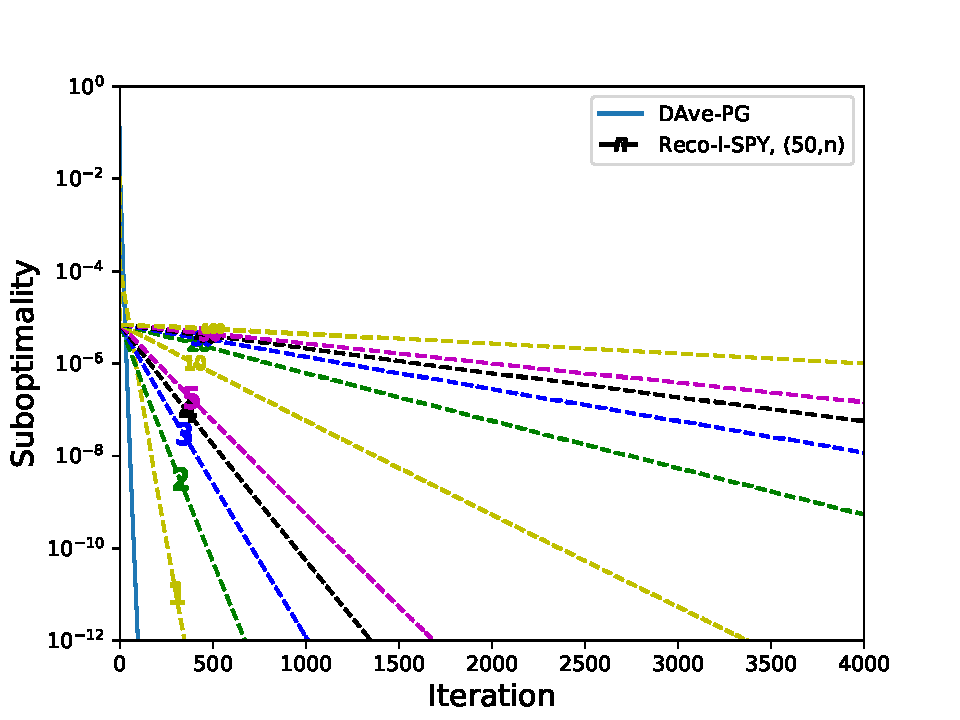
\includegraphics[width = 0.49\linewidth]{spy/figs/lasso_5w_1000_500_fun_vs_ite_log_coordinate.pdf}&
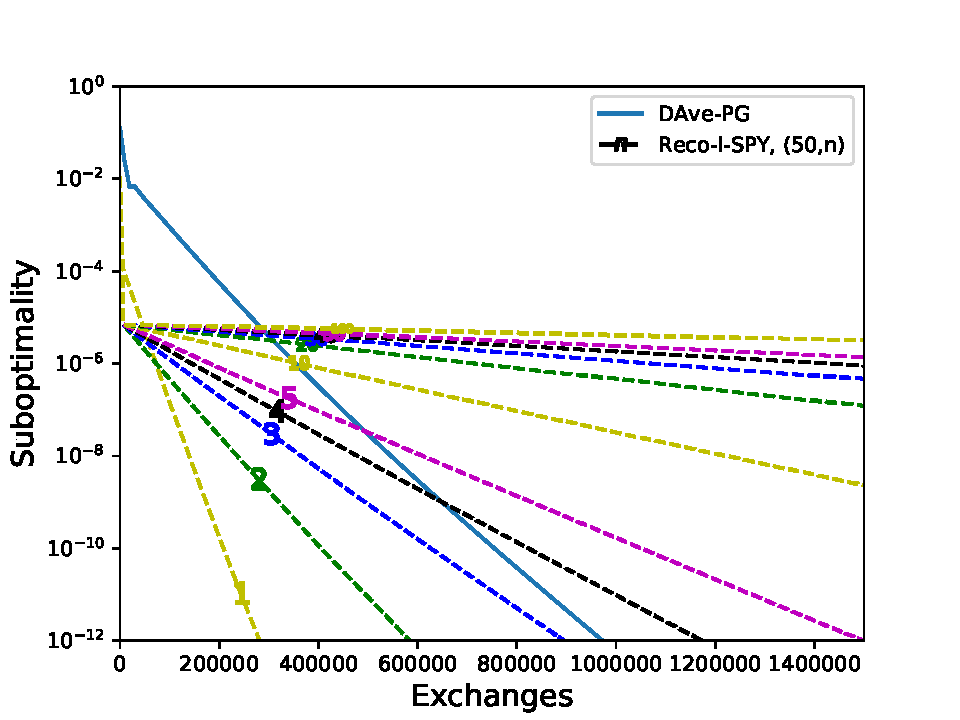
\includegraphics[width = 0.49\linewidth]{spy/figs/lasso_5w_1000_500_fun_vs_ex_log_coordinate.pdf}\\%\label{fig:real_f_vs_t}}
\end{tabular}
\caption{Dependence between convergence and the size of fixed budget on synthetic LASSO \eqref{eq:lasso}.}
\label{fig:fix_budget_variants}
\end{figure}
In Figure \ref{fig:fix_budget_variants}, we present the convergence of \recoalgo with fixed-budget stopping criteria on synthetic LASSO problem \eqref{eq:lasso} with $m=500$ and $n = 1000$. As we could see, the performance of the \recoalgo with $\mathsf{C}_1$ with fixed budget $\mathsf{M}_\ell\equiv 1$ is much better than for ones with inner cycle of bigger size. On the one hand, the theoretical budget criterion $\mathsf{C}_1$ propose \dg{the non-decreasing sequence $\mathsf{M}_{\ell}\geq1$}. On the other hand, as we could see from the plots, the slope is constant after some time, that means the rate of real $\mathsf{C}_1$ is expected to be slower than the algorithm run with $1$-epoch fixed budget and this is shown in Figure \ref{fig:fix_budget_variants_c1}. More precisely, we consider problem with $m=10000$ and $n=1000$ and as we could see, that the rate of $\mathsf{C}_1$ is worse and since lines contains horizontal parts the size of inner loop is bigger than it should be. We could see that algorithm with $\mathsf{C}_1$ is faster in identification in the beginning; however it needs much more time to identify the correct active-set in the end.
\begin{figure}[b!]
\begin{tabular}{cc}
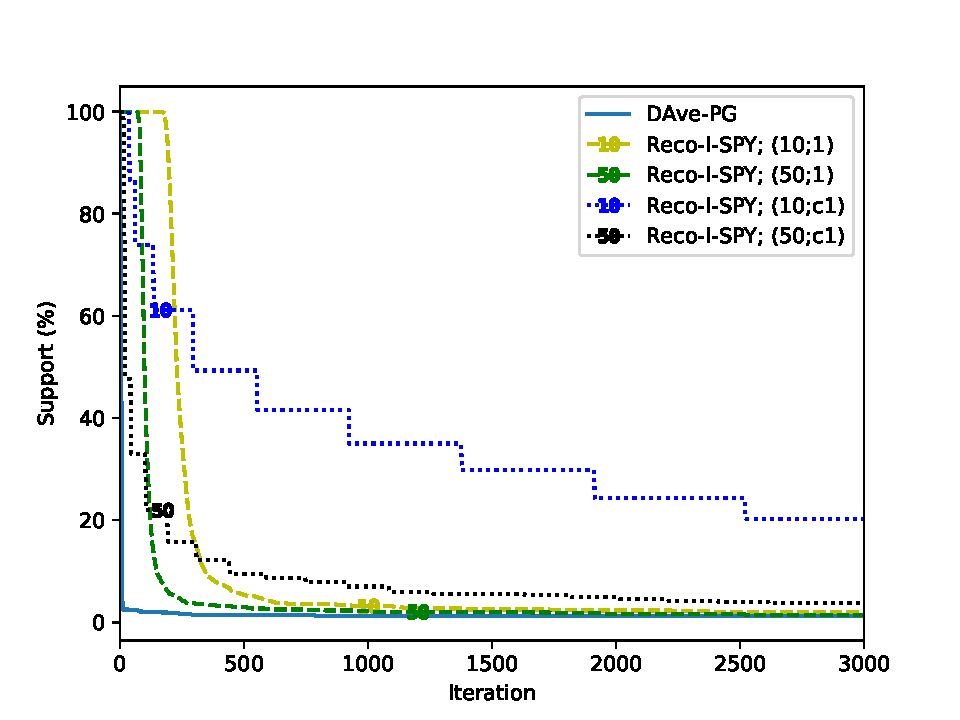
\includegraphics[width = 0.49\linewidth]{spy/figs/lasso_5w_1000_10000_density_criteria_1.pdf}&
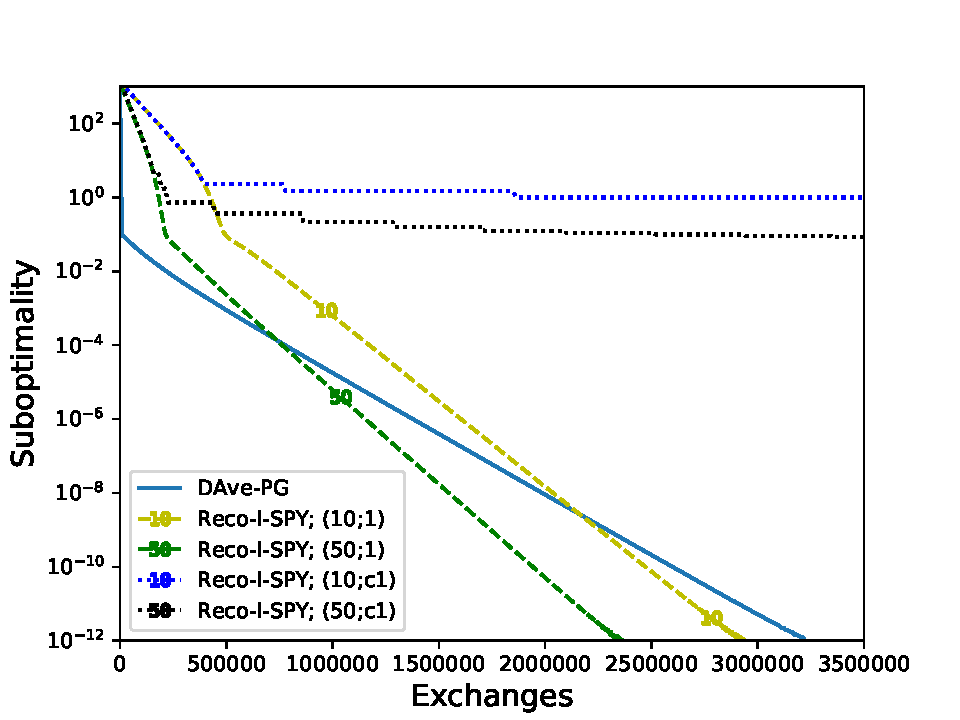
\includegraphics[width = 0.49\linewidth]{spy/figs/lasso_5w_1000_10000_fun_vs_ex_log_criteria_1.pdf}\\%\label{fig:real_f_vs_t}}
\end{tabular}
\caption{Synthetic LASSO \eqref{eq:lasso}: $1$-epoch vs $\mathsf{C}_1$.}
\label{fig:fix_budget_variants_c1}
\end{figure}


\subsubsection{Comparing with relative accuracy criterion}
Let us now consider the theoretical criterion $\mathsf{C}_3$. From the practical point of view this criterion is impossible to use since it requires the knowledge of the full dataset to verify. However, for us, it is important to make a comparison with it so we could see if the fixed budget mode is good enough in practice.

\paragraph{Criterion $\mathsf{C}_3$ for LASSO}

To verify the stopping criterion, we use the duality gap and the fact that the inner problem is convex and lower semi-continuous, we could bound the distance to the solution using the strong duality. We consider synthetic LASSO problem for which the solution of the dual problem could be explicitly computed from the primal solution.

In Figure \ref{fig:c3}, we see that the theoretical criterion $\mathsf{C}_3$ performs better in practice; however, the performance of $1$-epoch mode is worse only in the beginning since the duality gap does not give a tight approximation of the distance to the solution in general.
\begin{figure}[h!]
\begin{tabular}{cc}
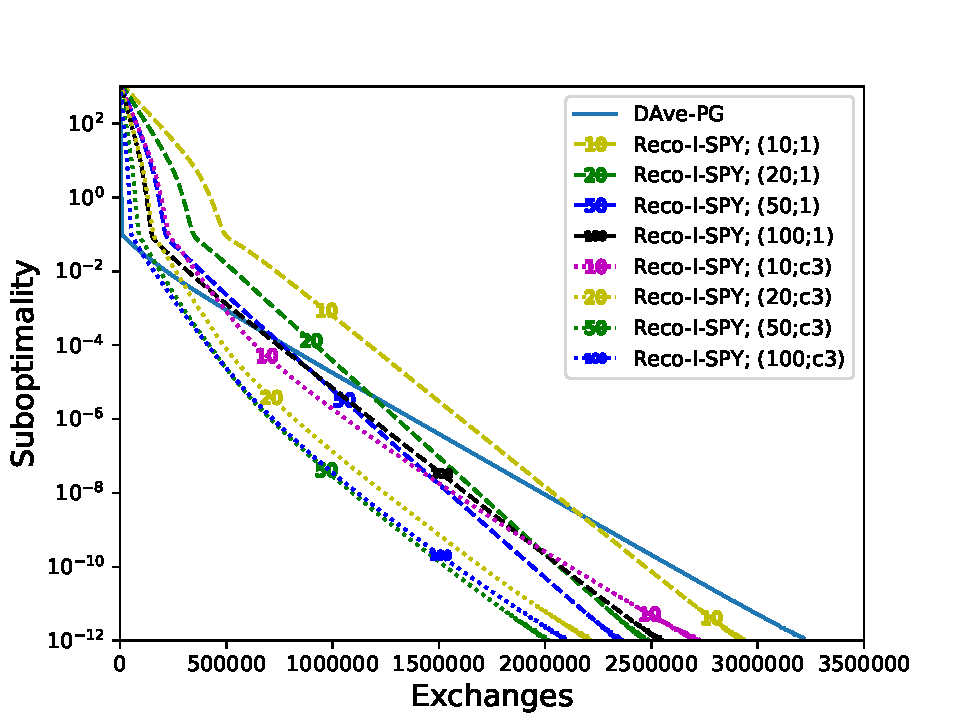
\includegraphics[width = 0.49\linewidth]{spy/figs/lasso_5w_1000_10000_fun_vs_ex_log_coordinate.pdf}&
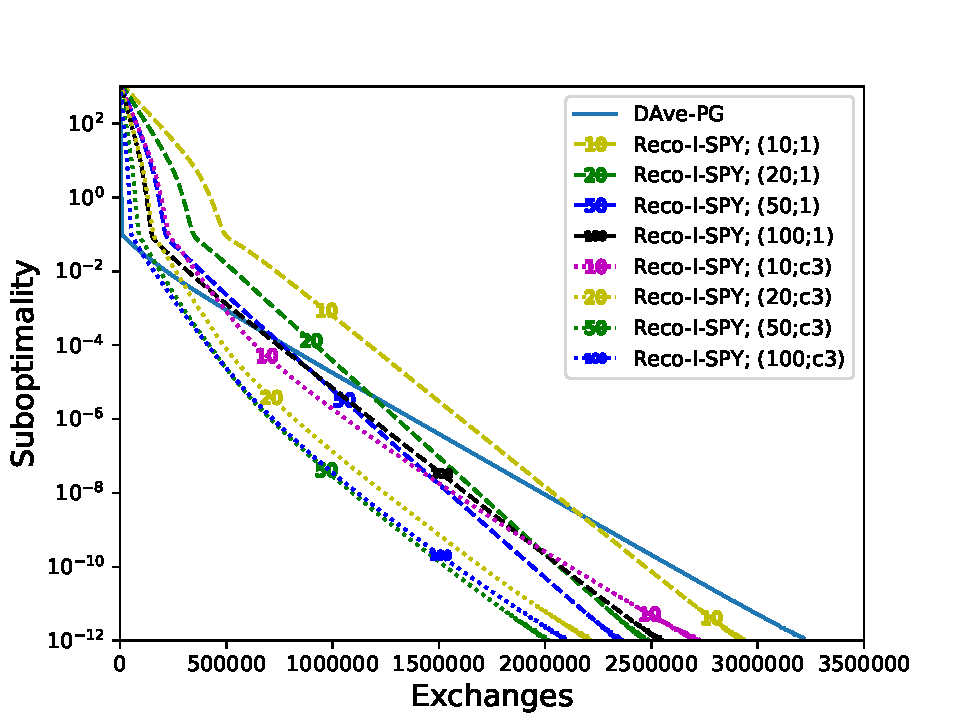
\includegraphics[width = 0.49\linewidth]{spy/figs/lasso_5w_1000_10000_fun_vs_ex_log_coordinate.pdf}\\%\label{fig:real_f_vs_t}}
\end{tabular}
\caption{Synthetic LASSO \eqref{eq:lasso}: $1$-epoch vs $\mathsf{C}_3$.}
\label{fig:c3}
\end{figure}

\paragraph{Criterion $\mathsf{C}_3$ for logistic regression}
Let us now consider logistic regression problem \eqref{eq:logistic2} where the dual solution is hard to compute. In this case, we use the following bound
\begin{align*}
    \|x_{\ell+1} - \prox_{F/\rho}(x_{\ell})\|_2\leq\frac{1}{\mu + \rho}\|\partial H_{\ell}(x_{\ell+1}) - \partial H_{\ell}(x_{\ell}^\star)\|_2\leq\frac{1}{\mu+\rho}\|\partial H_{\ell}(x_{\ell+1})\|_2.
\end{align*}
Since we use $\ell_1$ regularized problem the distance of subdifferential to $0$ is easy to compute; however, it requires full dateset to calculate it. This bound is less tight than duality gap one, so for practical experiments we use the stopping criterion
\begin{equation}\label{eq:c3_practice}
   \|\partial H_{\ell}(x_{\ell+1})\|^2_2\leq \frac{(\mu + \rho)^2\rho}{4(2\mu+\rho)(0.001\ell)^{2+2\delta}}\|x_{\ell+1}-x_{\ell}\|_2^2
\end{equation}

\begin{figure}[h!]
\begin{tabular}{cc}
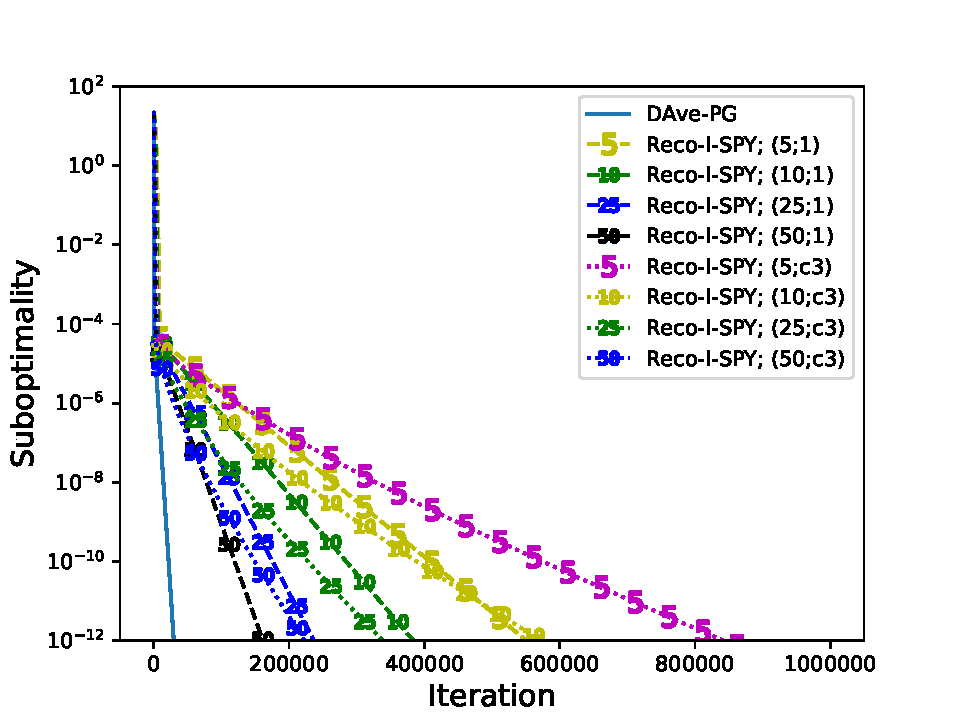
\includegraphics[width = 0.49\linewidth]{spy/figs/madelon_10w_003_0001_fun_vs_ite_log_c3.pdf}&
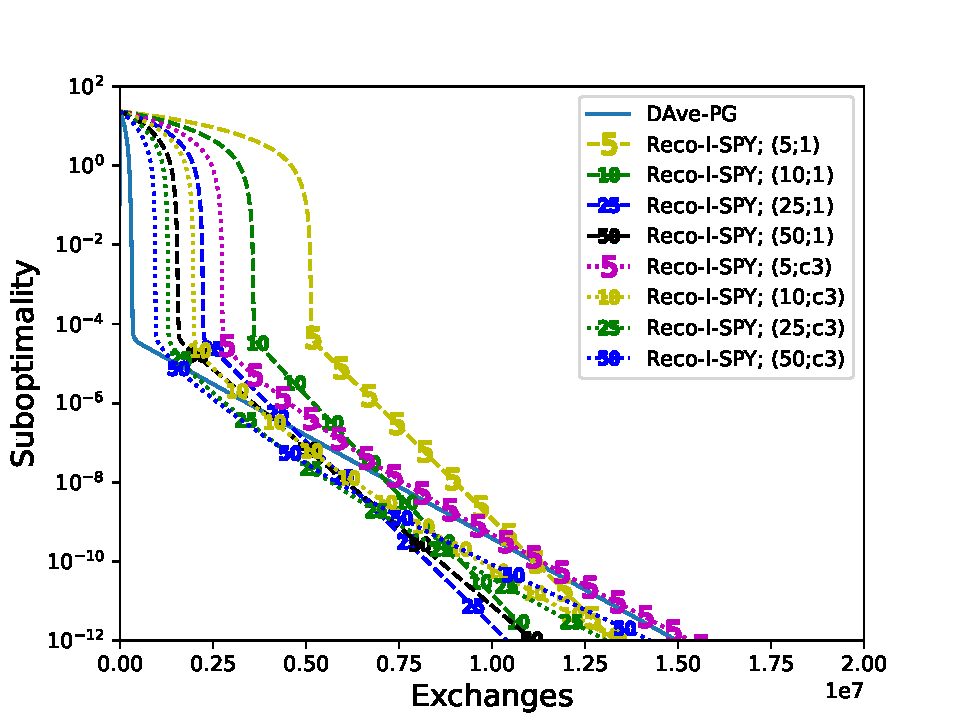
\includegraphics[width = 0.49\linewidth]{spy/figs/madelon_10w_003_0001_fun_vs_ex_log_c3.pdf}\\%\label{fig:real_f_vs_t}}
\end{tabular}
\caption{Logistic regression with elastic net regularization and madelon dataset: $1$-epoch vs $\mathsf{C}_3$.}
\label{fig:c3_log}
\end{figure}
In Figure \ref{fig:c3_log}, we present the performance of $1$-epoch mode versus $\mathsf{C}_3$ with the practical consideration as in \eqref{eq:c3_practice}. We consider logistic loss with elastic-net regularization on madelon dataset with $\lambda_1 = 0.03$ and $\lambda_2 = 0.001$. As we could see from the plots, the performance of such version of stopping criterion is worse than $1$-epoch mode in practice since the distance from the subdifferential to $0$ is not the best approximator; however, in the beginning, the performance of the theoretical run $\mathsf{C}_3$ is still better. 

\subsection{Warm start}
As we could see from the Figure \ref{fig:fix_budget_variants_c1}, the identification moment takes much more iterates for \recoalgo; however, there is no need to sparsify updates from the beginning since master-to-worker communication is not sparse. Considering this, we propose to run \dave~Algorithm first, for some amount of iterations and switch to \recoalgo when the current master point is sparse enough.

In Figure \ref{fig:rcv1_1epoch}, we present the experimental result for rcv1\_train dataset that has much more coordinates so that we could see the communication bottleneck in practice. 
\begin{figure}[h!]
\begin{tabular}{cc}
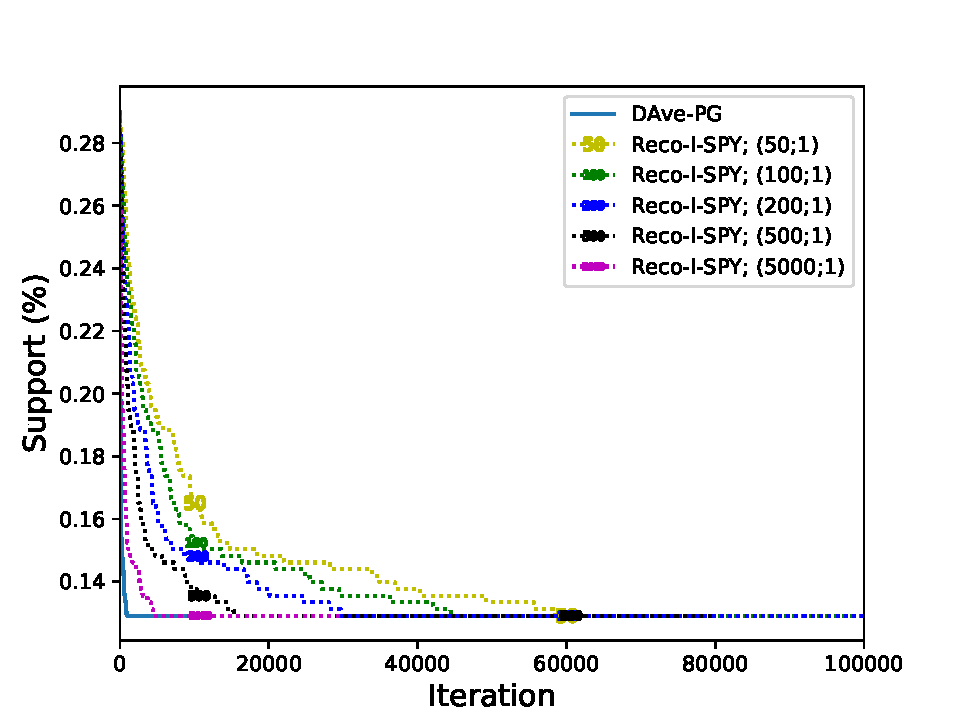
\includegraphics[width = 0.49\linewidth]{spy/figs/rcv1_train_20w_0001_00001_density.pdf}&
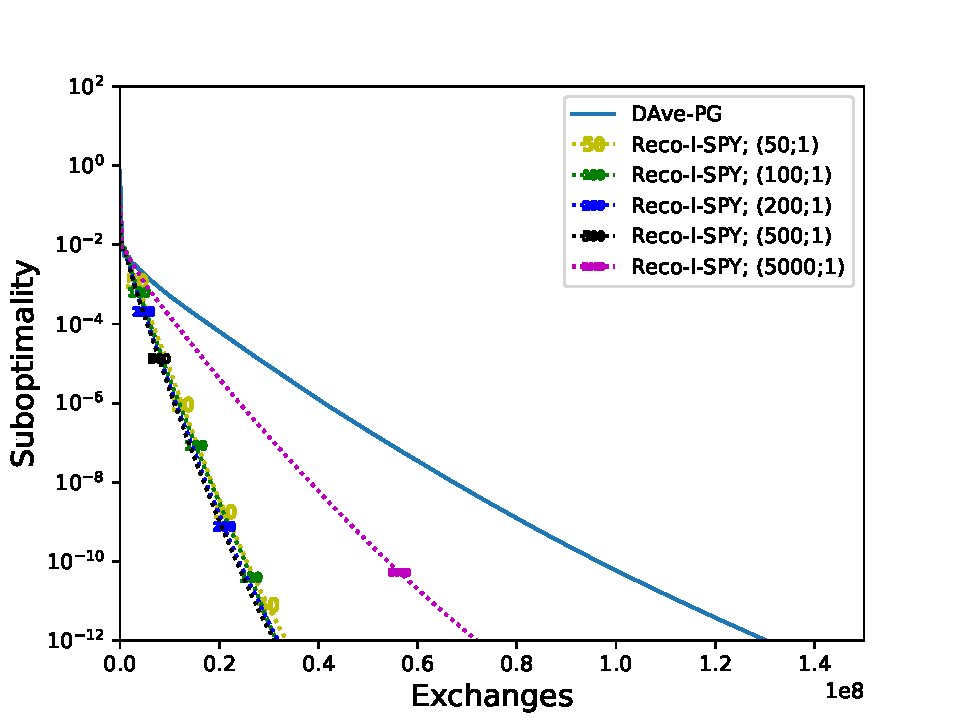
\includegraphics[width = 0.49\linewidth]{spy/figs/rcv1_train_20w_0001_00001_fun_vs_ex_log_coordinate.pdf}\\
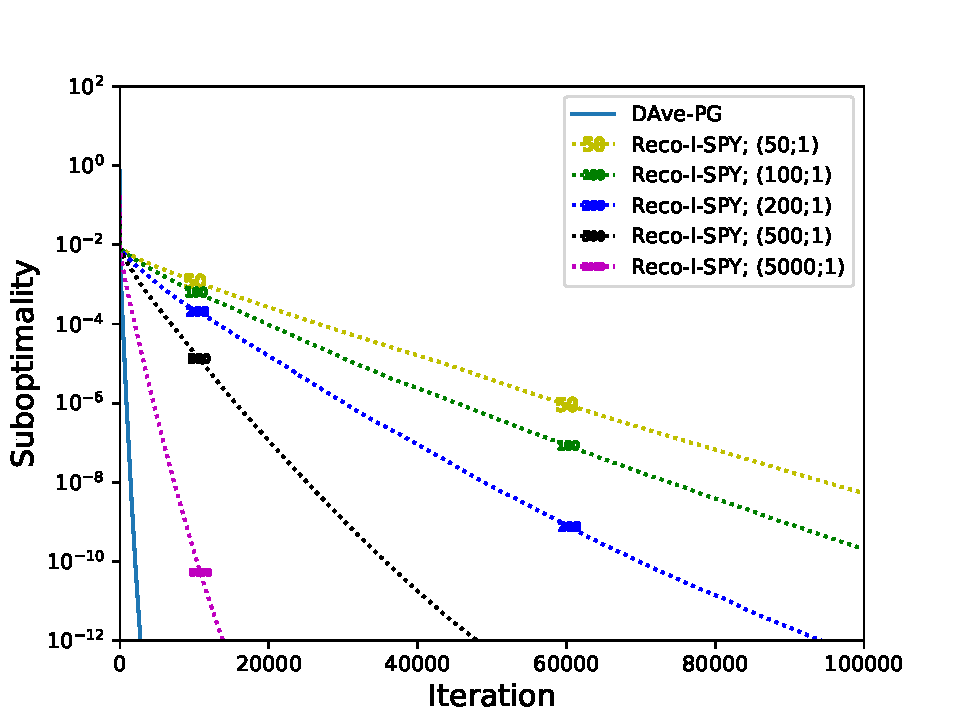
\includegraphics[width = 0.49\linewidth]{spy/figs/rcv1_train_20w_0001_00001_fun_vs_ite_log_coordinate.pdf}&
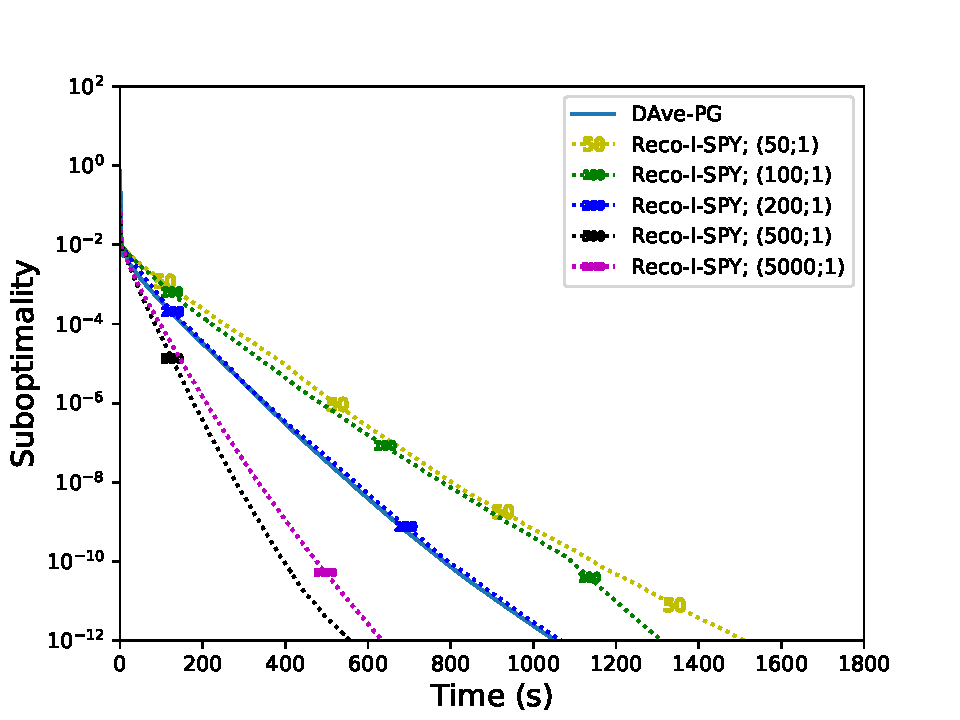
\includegraphics[width = 0.49\linewidth]{spy/figs/rcv1_train_20w_0001_00001_fun_vs_time_log.pdf}
\end{tabular}
\caption{Logistic regression with rcv1\_train dataset: $1$-epoch.}
\label{fig:rcv1_1epoch}
\end{figure}
More precisely, sparsified algorithm performs much better in terms of communication; however, the total amount of iterations is also sufficiently bigger for the very small $c$. As a result, the total time complexity is not well approximated by exchanges for $c\ll n$, that prevents us from using extreme sparsification that makes identification process and, as a result, convergence slower.


\section{Conclusion}
In this chapter, we present \recoalgo Algorithm that consists of two key components: \spyI~algorithm, that allows solving well-conditioned problems efficiently in terms of data exchanges and proximal reconditioning technique that allows solving the ill-conditioned problem via solving a sequence of well-conditioned subproblems iteratively. We present both the theoretical result and the performance in practice that both show that the sparsification technique helps to save runtime of the minimization process by decreasing the total amounts of bits sent.